% ===== UNIT 20: Comparison with the state of the art (5.1) =====
% Status: AI-DRAFT  (change to REWRITTEN / REVIEWED when done; see CHECKLIST.md)
% Rules: keep every \cite, \ref, \label, number and table value unless you checked it against the logs.
\subsection{Comparison with the state of the art}
Table~\ref{tab:sota} compares the proposed single-stream (S1) and fusion
results against published methods on VeRi-776, and Figure~\ref{fig:landscape}
places them in the mAP--Rank-1 landscape.

\begin{table*}[!t]
  \centering
  \caption{State-of-the-art comparison on VeRi-776.
    \cmark\,=\,post-processing (AQE / re-ranking) applied; \xmark\,=\,cosine
    similarity only. \emph{Rows differ in post-processing condition and are
    therefore not strictly like-for-like}: our pipeline rows are \cmark\ while
    several transformer baselines (TransReID, CLIP-ReID) are reported
    \xmark. Section~\ref{sec:matched} gives the matched-condition comparison}
  \label{tab:sota}
  \small
  \begin{tabular}{L{2.6cm}L{1.8cm}L{4.4cm}C{1.4cm}C{1.3cm}C{1.1cm}L{1.1cm}}
    \toprule
    Method & Venue & Backbone & mAP~(\%) & R1~(\%) & w/~PP & Ref. \\
    \midrule
    PROVID       & TMM 2018   & CNN (multi-modal)         & 53.42 & 81.56 & \xmark & \cite{liu2018provid} \\
    VAMI         & CVPR 2018  & CNN                       & 50.13 & 77.03 & \xmark & \cite{zhou2018vami} \\
    PVEN         & CVPR 2020  & ResNet50                  & 79.50 & 95.60 & \xmark & \cite{meng2020pven} \\
    HPGN         & T-ITS 2022 & CNN $+$ graph             & 80.18 & 96.72 & \xmark & \cite{shen2022hpgn} \\
    VehicleNet   & TMM 2020   & ResNet50                  & 83.41 & 96.78 & \cmark & \cite{zheng2020vehiclenet} \\
    TransReID    & ICCV 2021  & DeiT-B/16                 & 82.30 & 97.10 & \xmark & \cite{he2021transreid} \\
    CLIP-ReID    & AAAI 2023  & ViT-B/16                  & 84.50 & 97.30 & \xmark & \cite{li2023clipreid} \\
    RPTM         & WACV 2023  & ResNet                    & 88.00 & 97.30 & \xmark & \cite{ghosh2023rptm} \\
    MBR4B-LAI    & ITSC 2023  & ResNet50 (multi-branch)   & 92.09 & 98.03 & \cmark & \cite{luo2023mbr4b} \\
    CLIP-SENet   & arXiv 2025 & ResNet101-IBN-a $+$ TinyCLIP & 92.90 & 98.70 & \cmark & \cite{lu2025clipsenet} \\
    \midrule
    \textbf{Ours (S1, w/ PP)} & ---  & ViT-B/16 (CLIP init.) & \textbf{89.97} & \textbf{97.79} & \cmark & --- \\
    \textbf{Ours (fusion)}    & ---  & ViT-B $+$ ResNet101-IBN-a $+$ TinyCLIP & \textbf{93.32} & \textbf{98.45} & \cmark & --- \\
    \bottomrule
  \end{tabular}
\end{table*}

\begin{figure}[!t]
  \centering
  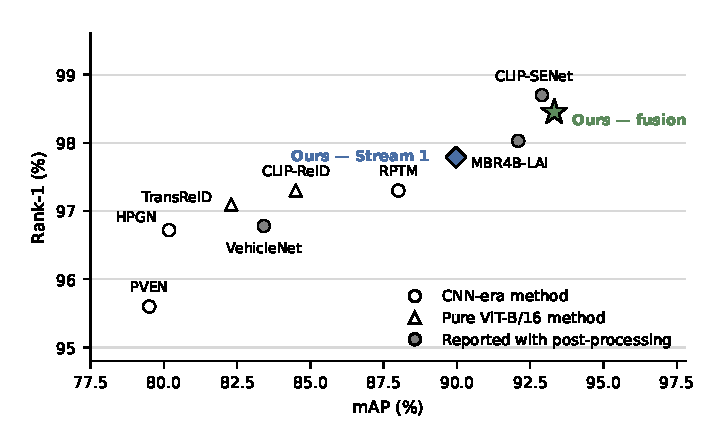
\includegraphics[width=0.92\columnwidth]{Fig3}
  \caption{Published VeRi-776 results in the mAP--Rank-1 plane. Filled markers
  denote results reported with post-processing; open markers denote
  raw-embedding results. Early CNN-era methods (PROVID, 53.4\% mAP; VAMI,
  50.1\% mAP) fall outside the plotted range and are omitted for readability.
  The single-stream result of this work is competitive but, as
  Section~\ref{sec:matched} shows, this reflects post-processing rather than a
  recipe advantage}
  \label{fig:landscape}
\end{figure}

This table should be read with care, because the rows mix post-processing
conditions. First, our ViT-B pipeline (89.97\% mAP, \cmark) is the strongest
\emph{pure-ViT-B} entry \emph{among published results}, but those baselines are
reported \emph{without} post-processing (\xmark); when we apply our identical
post-processing to the official TransReID and CLIP-ReID checkpoints they reach
91.12\% and 91.80\% mAP, both \emph{exceeding} ours
(Section~\ref{sec:matched}), so this row reflects post-processing rather than a
recipe advantage. Among single models reported \emph{with} post-processing,
MBR4B-LAI (92.1\% mAP~\cite{luo2023mbr4b}) also exceeds our single stream.
Second, the fusion (93.32\% mAP) marginally exceeds the best prior published
result (CLIP-SENet, 92.9\%~\cite{lu2025clipsenet}) by $+0.42$\,pp and
MBR4B-LAI by $+1.23$\,pp, which we interpret as evidence of stream
complementarity rather than a decisive margin.
